\documentclass[]{article}

%\usepackage[authoryear]{natbib}
%\usepackage[round,sort&compress,sectionbib]{natbib}

\usepackage[style=authoryear,maxnames=5,backend=bibtex,natbib=true]{biblatex}
%\bibliographystyle{plain}
\addbibresource{AIP-GalClusTurb.bib}

%\bibliographystyle{plainnat}
\usepackage{hyperref}
\usepackage{siunitx}
\usepackage{bm}
\let\vec\bm
\usepackage{xurl}
\usepackage{subcaption}
\usepackage{graphicx}   % Including figure files
\usepackage{amsmath}   % Advanced maths commands
\usepackage{amssymb}   % Extra maths symbols
\usepackage{xcolor}
\usepackage[makeroom]{cancel}
%\usepackage{soul}
\newcommand{\mathcolorbox}[2]{\colorbox{#1}{$\displaystyle #2$}}
\colorlet{lgray}{gray!50!white}
\colorlet{lred}{red!50!white}
\newcommand{\bnabla}{\bm{\nabla}}
\newcommand{\bcdot}{\bm{\cdot}}
\newcommand{\ud}{\,\mathrm{d}}


%opening
\title{Energy flux}
\author{Lorenzo M. Perrone, TB, EP, CP}

\begin{document}

\maketitle

\begin{abstract}
In this document we derive the evolution equation for the large-scale and small-scale kinetic/magnetic energy and the energy fluxes.
\end{abstract}

\section{Ideal MHD equations}

We neglect viscous/resistive dissipation (the additional terms are easy to handle).

\begin{align}
	\frac{\partial \rho}{\partial t} + \nabla \bcdot \left(\rho \bm u \right) = 0, \\
	\frac{\partial }{\partial t} \left(\rho \bm u \right) + \nabla \bcdot \left( \rho \bm u \bm u  + p_{\mathrm{tot}} \mathbb{I}  - \frac{\bm B \bm B}{4 \pi} \right) = - \rho \nabla \Phi , \\
	\frac{\partial \bm B}{\partial t} = \nabla \times \left( \bm u \times \bm B \right), \\
	\frac{\partial p}{\partial t} + \bm u \bcdot \nabla p + \gamma p \nabla \bcdot \bm u = 0, \label{eq:thermal_pressure}
\end{align}
%
where $p_{\mathrm{tot}} = p + B^2 / 8\pi$, and $p$ is the thermal pressure. 

\section{Definitions}

Classically smoothed field: $\langle \bm u \rangle$. Favre averaging: $\tilde{\bm u} \equiv \langle \rho \bm u \rangle / \langle \rho \rangle$. The second order statistical moment is defined as
%
\begin{align}
	\mu_2 (f, g) = \langle f g \rangle - \langle f \rangle \langle g \rangle.
\end{align}
%
The term $\tilde{\mu}_2 (u_i, u_j)$ is a shorthand for
%
\begin{align}
	\tilde{\mu}_2 (u_i, u_j) \equiv \widetilde{u_i u_j} - \tilde{u}_i \tilde{u}_j.
\end{align}
%
To simplify the notation we will interchangeably use $\langle f \rangle = \overline{f}$.

\section{Large-scale evolution}

\subsection{Kinetic energy}

With Favre-averaging, the large-scale kinetic energy is defined as $\overline{\rho} \tilde{\bm u}^2 / 2$. Its evolution is given by:
%
%\begin{align}
%	&\partial_t \left( \frac{\overline{\rho} \tilde{\bm u}^2}{2} \right) + \partial_j \left[ \left( \frac{\overline{\rho} \tilde{\bm u}^2}{2} + \langle p_{\mathrm{tot}} \rangle \right) \tilde{u}_j + \tilde{u}_i \overline{\rho} \left( \tilde{\mu}_2 (u_i, u_j) - \frac{\mu_2 (B_i, B_j)}{4\pi} \right) \right. \nonumber \\
%	&\left. - \frac{1}{4\pi} \tilde{u}_i \langle B_i \rangle \langle B_j \rangle   \right] = \overline{\rho} \tilde{\mu}_2 (u_i, u_j) \partial_j \tilde{u}_i - \frac{1}{4\pi} \mu_2 (B_i, B_j) \partial_j \tilde{u}_i \nonumber \\ 
%	&- \frac{1}{\overline{\rho}} \mu_2 (\rho, u_i) \partial_i \langle p_{\mathrm{tot}} \rangle + \langle p_{\mathrm{tot}} \rangle \partial_i \langle u_i \rangle - \frac{1}{4\pi} \langle B_i \rangle \langle B_j \rangle  \partial_j \tilde{u}_i
%\end{align}
%%
%Can be rewritten as:
\begin{align}\label{eq:large-scale-kin-en}
	&\partial_t \left( \frac{\overline{\rho} \tilde{\bm u}^2}{2} \right) + \nabla \bcdot \bm F^K = - \Pi^K_{\ell} - \Lambda_{\ell} - Q_{\ell}  - T_{\ell} - G_{\ell} - \tilde{\bm u} \bcdot \overline{\rho \nabla \Phi} . 
\end{align}
%
In the previous expression $\bm F^K$ is the spatial transport: 
\begin{align}
	(F^K)_j = \left( \frac{\overline{\rho} \tilde{\bm u}^2}{2}  \right) \tilde{u}_j +  \overline{\rho} \tilde{u}_i \tau_{ij} + \overline{p}_{\mathrm{tot}} \overline{u}_j - \frac{\overline{B}_i \overline{B}_j}{4\pi} \overline{u}_i  
\end{align}
where $\tau_{ij}$ is the total (Reynolds plus Maxwell) small-scale stress tensor:
\begin{align}
	\tau_{ij} \equiv \tilde{\mu}_2 (u_i, u_j) - \frac{\mu_2 (B_i, B_j)}{4\pi \overline{\rho}} .
\end{align}
%
On the right-hand side we have sinks and sources of large-scale kinetic energy. $\Pi^K_{\ell}$ is the subgrid scale (SGS) flux:
\begin{align}\label{eq:sgs_term}
	\Pi^K_{\ell} = - \overline{\rho} \tau_{ij} \partial_i \tilde{u}_j
\end{align}
%
$\Lambda_{\ell}$ is called baropycnal work (large-scale pressure gradient and magnetic tension acting on turbulent mass flux):
\begin{align}\label{eq:baropycnal_term}
	\Lambda_{\ell} = \frac{1}{\overline{\rho}} \mu_2 (\rho, u_i) \partial_j \left( \overline{p}_{\mathrm{tot}} \delta_{ij} -  \frac{\overline{B}_i \overline{B}_j}{4\pi} \right)
\end{align}
%
$Q_{\ell}$ is called large-scale pressure dilatation (converts large-scale energy from kinetic to thermal): 
\begin{align}\label{eq:largescale_press_dil_term}
	Q_{\ell} = - \overline{p} \partial_i  \overline{u}_i . 
\end{align}
$T_{\ell}$ is the kinetic energy expended by the large-scale flow to bend and stretch large-scale magnetic field including adiabatic compression:
%
\begin{align}\label{eq:largescale_mag_stretch_term}
	T_{\ell} = \frac{1}{4\pi} \overline{B}_i \overline{ B}_j   \partial_j \overline{u}_i - \frac{\overline{B}^{2}}{8\pi} \partial_i  \overline{u}_i ,
\end{align}
%
and $G_{\ell}$ is the adiabatic compression of small-scale magnetic energy by the large-scale flow:
%
\begin{align}\label{eq:adiab_compress_small_mag_largescale}
	G_{\ell} = -  \frac{\mu_2 (B_i, B_i)}{4\pi} \partial_i  \overline{u}_i . 
\end{align}
%
Of the terms in Eq.~\eqref{eq:large-scale-kin-en}, only $\Pi^K_{\ell}$ (Eq.~\ref{eq:sgs_term}), $\Lambda_{\ell}$ (Eq.~\ref{eq:baropycnal_term}) and $G_{\ell}$ (Eq.~\ref{eq:adiab_compress_small_mag_largescale}) can transfer energy across scales, since they physically describe large-scale fields acting against small-scale fluctuations. In particular, $\Pi^K_{\ell}$ and $\Lambda_{\ell}$ describe kinetic energy flux from large to small scales, while $G_{\ell}$ converts energy between large-scale kinetic energy and small-scale magnetic energy.
On the other hand, large-scale pressure dilatation $Q_{\ell}$ (Eq.~\ref{eq:largescale_press_dil_term}) and the large-scale magnetic stretching $T_{\ell}$ (Eq.~\ref{eq:largescale_mag_stretch_term}) only involve large-scale fields, and therefore cannot transfer energy across scales.


\subsection{Magnetic energy}

The large-scale magnetic energy is defined as $\overline{\bm B}^2 / 8\pi$. Its evolution is given by:
%
\begin{align}
	\partial_t \left( \frac{\overline{\bm B}^2}{8\pi}\right) + \nabla \bcdot \bm F^{B} = - \Pi^B_{\ell} + T_{\ell} ,
\end{align}
%
where $\bm F^{B}$ is the large-scale magnetic spatial transport:
\begin{align}
	\bm F^{B} &= \frac{\overline{\bm B}^2}{8\pi} \overline{\bm u} - c\frac{\overline{\bm  \epsilon} \times \overline{\bm B}}{4 \pi} \nonumber \\
	&= \frac{\overline{\bm B}^2}{8\pi} \overline{u}_j - \overline{B}_i \left( \frac{\mu_2 (u_i, B_j)}{4\pi} - \frac{\mu_2 (u_j, B_i)}{4\pi} \right),
\end{align}
%
where $c \overline{\bm  \epsilon} \equiv \overline{\bm u \times \bm B} - \overline{\bm u} \times \overline{\bm B}$ is the small-scale emf, and $\Pi^B_{\ell}$ is the subgrid-scale SGS magnetic flux:
%
\begin{align}
	\Pi^B_{\ell} &= - \overline{\bm  \epsilon} \bcdot \overline{\bm J} \nonumber \\
	&= \left( \frac{\mu_2 (u_i, B_j)}{4\pi} - \frac{\mu_2 (u_j, B_i)}{4\pi} \right) \partial_j \overline{B}_i ,
\end{align}
%
where $\overline{\bm J} = (c/ 4\pi) \nabla \times \overline{\bm B}$ is the large-scale electric current. Finally, $T_{\ell}$ is the same as in Eq.~\eqref{eq:large-scale-kin-en}, and represents stretching of large-scale magnetic field (Eq.~\ref{eq:largescale_mag_stretch_term}) appearing now with opposite sign.


\section{Small-scale evolution}

\subsection{Kinetic energy}

With Favre-averaging the small-scale kinetic energy is defined as $\overline{\rho} \tilde{\mu}_2 (u_i, u_i) / 2$. Its evolution is given by:
%
\begin{align}
	\partial_t \left( \frac{\overline{\rho} \tilde{\mu}_2 (u_i, u_i)}{2}\right) + \nabla \bcdot \bm f^K &= \Pi^K_{\ell} + \Lambda_{\ell} + \mu_2 \left(p, \nabla \bcdot \bm u\right) + \mu_2 \left( \frac{B^2}{8 \pi}, \nabla \bcdot \bm u \right) \nonumber \\
	&- S_{\ell} - \overline{\rho} \tilde{\mu}_2 (u_i, \partial_i \Phi).
\end{align}
%
The small-scale kinetic spatial transport term $\bm f^{K}$ is:
%
\begin{align}
	(f^{K})_j &= \frac{1}{2} \overline{\rho} \tilde{\mu}_2 (u_i, u_i) \tilde{u}_j + \frac{1}{2} \overline{\rho} \tilde{\mu}_3 (u_i, u_i, u_j) + \mu_2 (p_{\mathrm{tot}}, u_j) + \frac{\mu_2 (B_i, B_j) }{4\pi}\tilde{u}_i \nonumber \\
	&- \left( \frac{\overline{B_i B_j u_i}}{4\pi} - \frac{\overline{B}_i \overline{B}_j \overline{u}_i}{4\pi} \right).
\end{align}
%
On the right-hand side we find again the kinetic subgrid scale flux $\Pi^K_{\ell}$ (Eq.~\ref{eq:sgs_term}), and the baropycnal work $\Lambda_{\ell}$ (Eq.~\ref{eq:baropycnal_term}), this time with opposite sign with respect to Eq.~\eqref{eq:large-scale-kin-en}. The two terms $ \mu_2 \left(p, \nabla \bcdot \bm u\right) + \mu_2 \left( B^2 /8 \pi, \nabla \bcdot \bm u \right)$ involve small-scale exchange between kinetic and thermal (magnetic) energy, respectively. 
The term $S_{\ell}$ is the small-scale stretching of magnetic fields:
%
\begin{align}
	S_{\ell} = \left( \frac{\overline{B_i B_j \partial_j u_i}}{4\pi} - \frac{\overline{B}_i \overline{B}_j \partial_j \overline{u}_i}{4\pi} \right),
\end{align}
%
and finally the last term $- \overline{\rho} \tilde{\mu}_2 (u_i, \partial_i \Phi)$ is the conversion between small-scale gravitational and kinetic energy.

\subsection{Magnetic energy}

The small-scale magnetic energy is defined as $ \mu_2 (B_i, B_i) / 8 \pi$. Its evolution is given by:
%
\begin{align}\label{eq:small-scale-mag-energy}
	\partial_t \left( \frac{\mu_2 (B_i, B_i)}{8 \pi} \right) + \nabla \bcdot \bm f^B = \Pi^B_{\ell} + S_{\ell} + G_{\ell}  - \mu_2 \left( \frac{B^2}{8 \pi}, \nabla \bcdot \bm u \right),
\end{align}
%
where $\bm f^B$ is the spatial transport of small-scale magnetic energy
%
\begin{align}
	(f^B)_j = \frac{\mu_2 (B_i, B_i)}{8 \pi} \overline{u}_j + \frac{\mu_3 (B_i, B_i, u_j)}{8 \pi} + \overline{B}_i \frac{\mu_2 (u_i, B_j)}{4 \pi} ,
\end{align}
%
and where on the right-hand side of Eq.~\eqref{eq:small-scale-mag-energy} we find as sources the subgrid scale magnetic flux $\Pi^B_{\ell}$, the small-scale stretching $S_{\ell}$, the adiabatic compression of small-scale magnetic energy by the large-scale flow $G_{\ell}$, and finally the small-scale kinetic to magnetic exchange $- \mu_2 \left( B^2/8 \pi, \nabla \bcdot \bm u \right)$.

\section{Internal energy}

Filtering the equation for thermal pressure (Eq.~\ref{eq:thermal_pressure}) we obtain the evolution equation for the mean internal energy $\overline{\rho e} = \overline{p} / (\gamma - 1)$:
%
\begin{align}\label{eq:internal_energy}
	\partial_t \left( \frac{\overline{p}}{\gamma - 1}\right) + \nabla \bcdot \left( \frac{\overline{p}}{\gamma - 1} \overline{\bm u} + \frac{\mu_2 ( p, \bm u )}{\gamma - 1} \right) = Q_{\ell} - \mu_2 (p, \nabla \bcdot \bm u).
\end{align}
%
We stress that $\overline{\rho e} = \overline{p} / (\gamma - 1)$   is \textit{not} the large-scale internal energy: indeed, integrating Eq.~\ref{eq:internal_energy} over the volume we get the total internal energy contained therein (because the operation of filtering and averaging commute). One might define $\bar{\rho} \bar{e}$ as the large-scale internal energy, and $\mu_2 (\rho, e)$ as the small-scale internal energy (such that their sum yields $\overline{\rho e}$) but (a) I have not seen it in the literature, and (b) it is not necessary for our purposes.


\begin{figure}
	\centering
	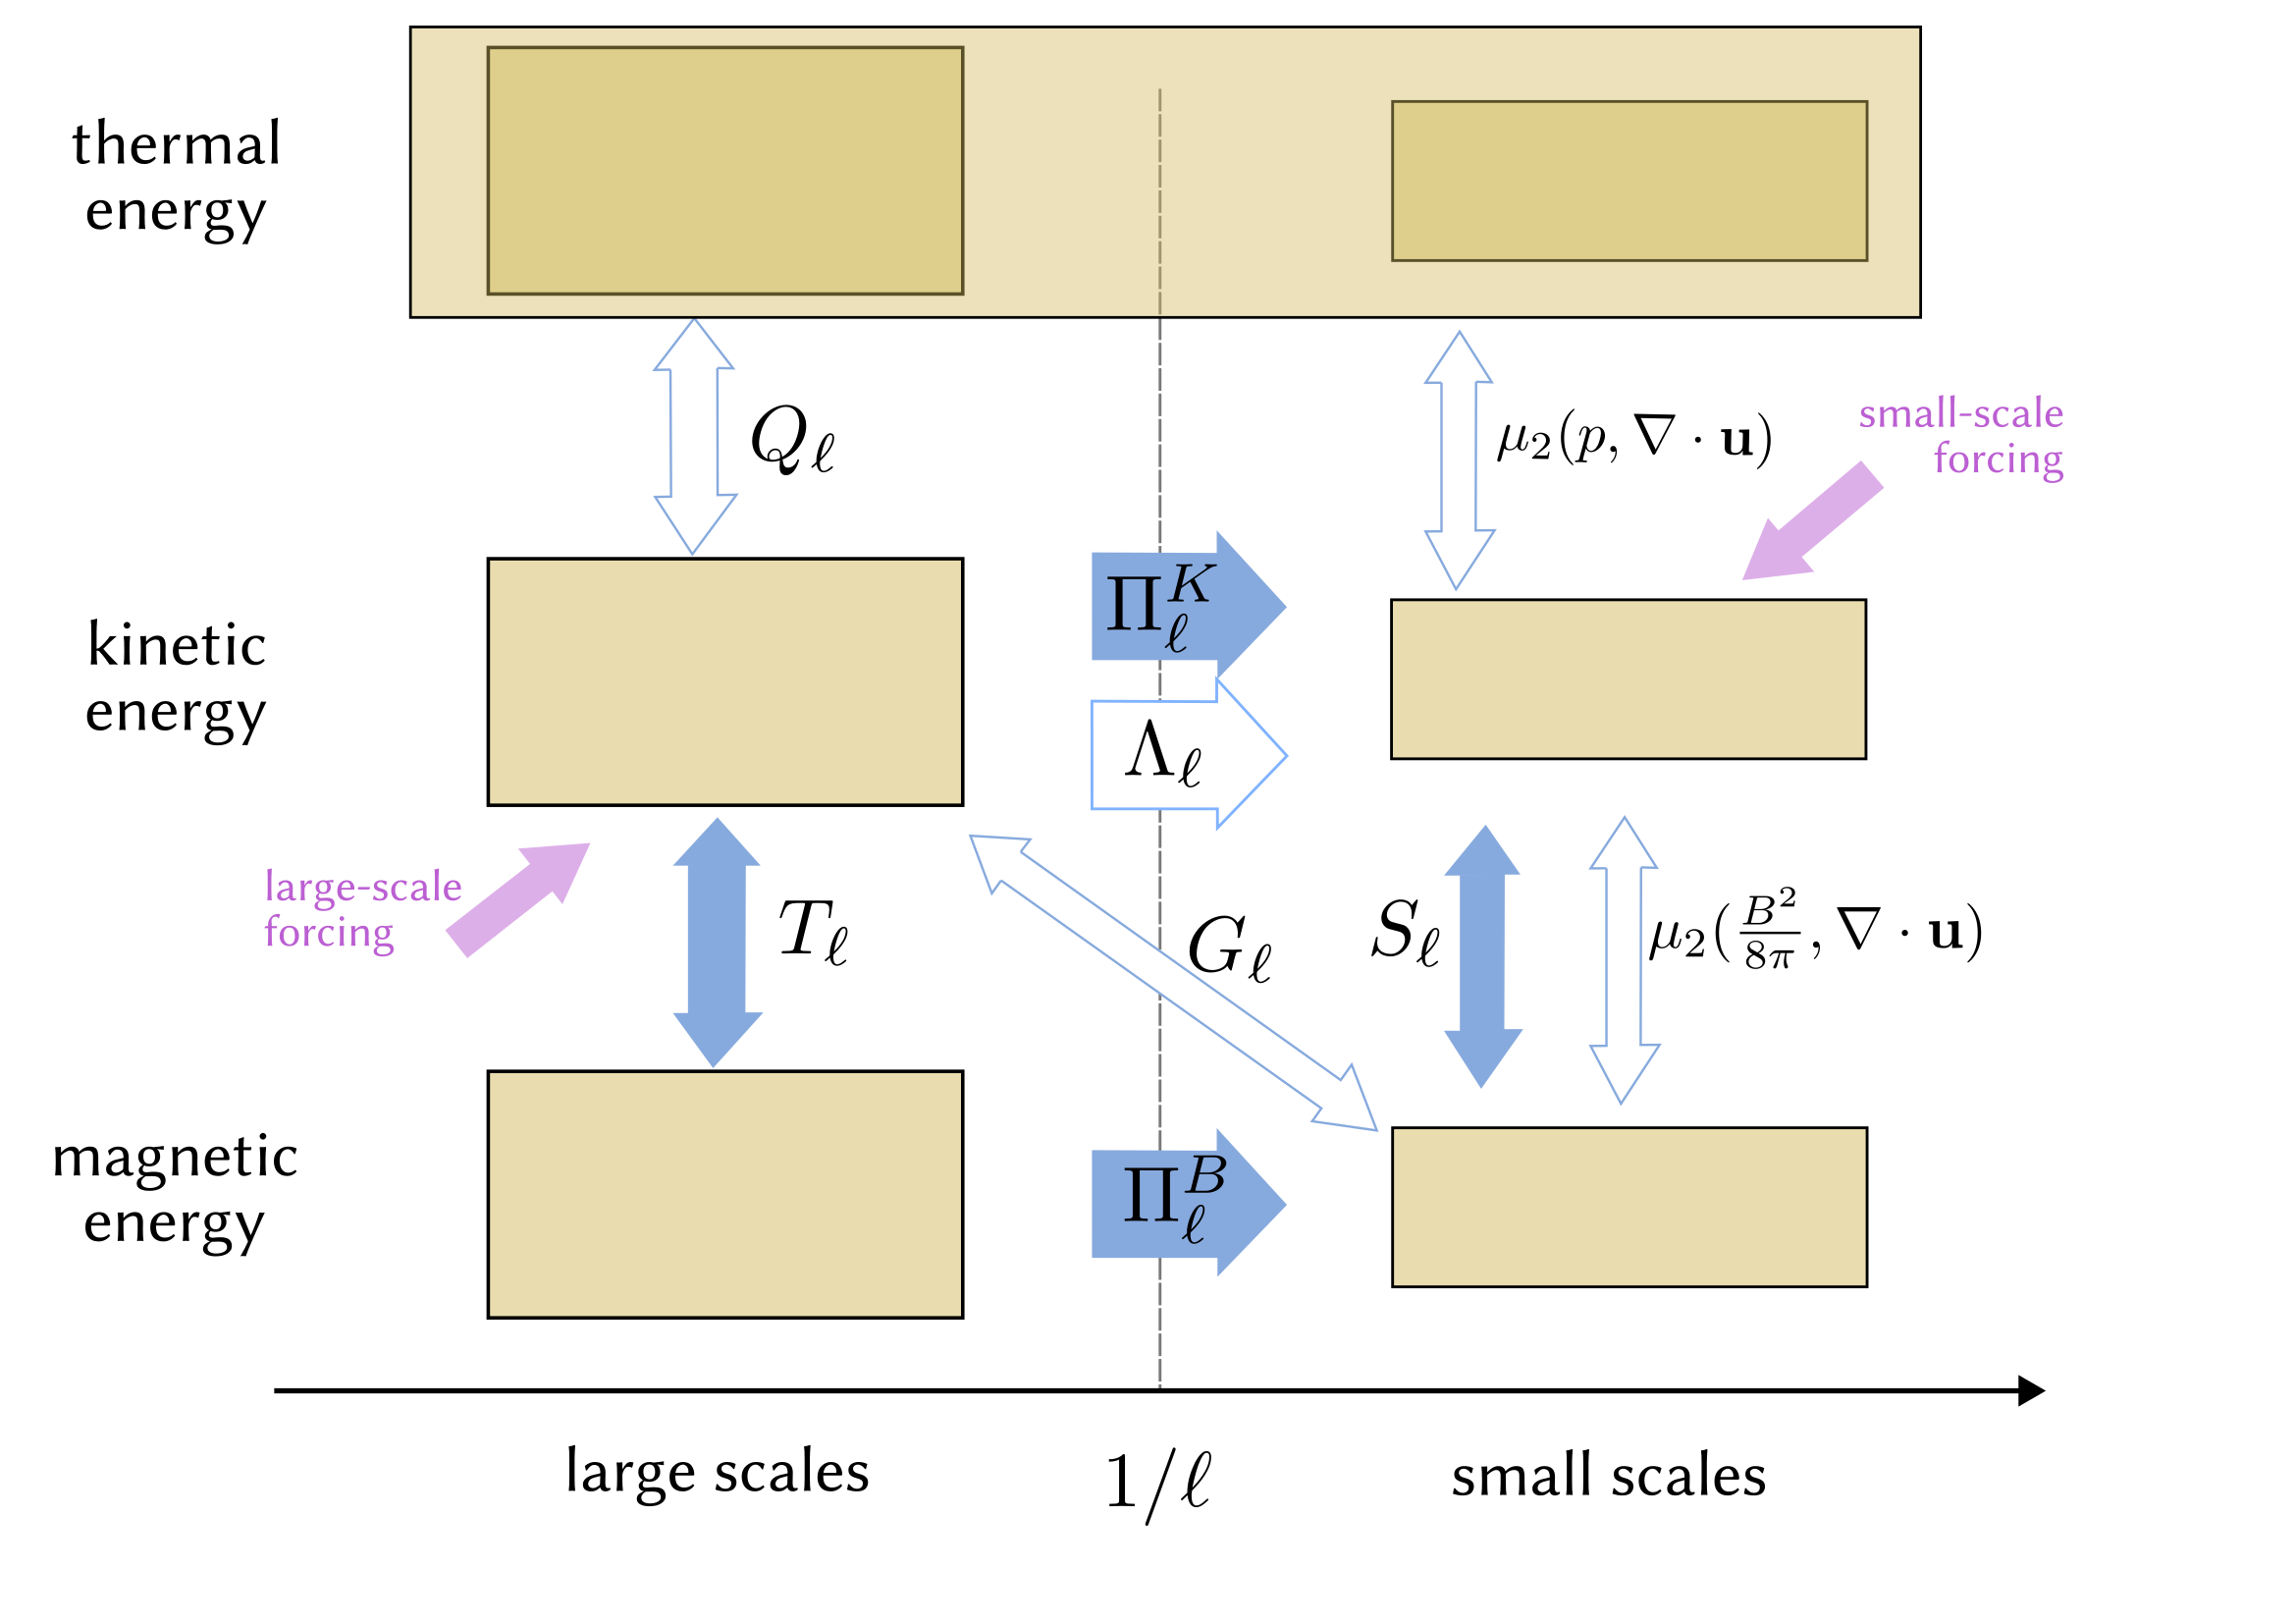
\includegraphics[width=1.0\linewidth]{Figures/mhd_fluxes.png}
	\caption{Representation of energy fluxes and transfers in ideal compressible MHD. Empty arrows represent terms solely due to compressibility. Note, however, that compressibility effects also contribute to $\Pi^K_{\ell}$, $T_{\ell}$ and $S_{\ell}$ (because of the velocity shear matrix).}
	\label{fig:kin_pot_mag_energy}
\end{figure}



%\printbibliography

\end{document}
